\RequirePackage[T1]{fontenc}
\documentclass[conference,letterpaper,10pt]{IEEEtran}
\usepackage[T1]{fontenc}
\usepackage{mathptmx}
\usepackage{amsmath,amssymb}
\usepackage{graphicx}
\usepackage{booktabs,array,tabularx}
\usepackage{float}
\usepackage{xcolor}
\usepackage{url}
\usepackage[hidelinks]{hyperref}
\usepackage{cite}
\graphicspath{{figures/}}
\newcommand{\E}{\mathbb{E}}
\newcommand{\ind}{\mathbf{1}}
\newcommand{\conpath}{ConPath}
\newcommand{\valonly}{\textbf{Development validation only.}}
\newcommand{\workingnote}{\begin{center}\small\textbf{Anonymous working draft --- 10 September 2026}\\Validation-only evidence; not a submission-ready or final-test report.\end{center}}
\setlength{\emergencystretch}{1em}
\renewcommand{\arraystretch}{1.12}
\renewcommand{\topfraction}{0.85}
\renewcommand{\dbltopfraction}{0.85}
\renewcommand{\textfraction}{0.1}
\pagestyle{plain}

\title{ConPath: Joint Spatial Map Posteriors for\\Footprint-Aware Reachability Prediction}
\author{\IEEEauthorblockN{Anonymous working draft}}
\begin{document}
\maketitle
\workingnote

\begin{abstract}
A robot's ability to reach a goal through partly observed space depends on how free cells occur together, as well as on their individual probabilities. We study the probability that a path exists for a specified circular footprint, conditioned on a partial bird's-eye-view map and a supplied valid-support mask. ConPath represents a joint stochastic occupancy posterior with global latent factors and local spatial noise, conditions sampled worlds to preserve observed evidence under the registered sampling rule, and estimates reachability by exact disk erosion and connectivity. A sample-pair event objective trains the posterior toward the downstream forecast. On a small FlatLands development split with disjoint parent places, three seeds obtain Event Brier 0.10380 versus 0.11201 for independently sampled completion. A separate historical intervention preserves every empirical cell marginal while increasing Event Brier from 0.06749 to 0.16139 after spatial dependence is disrupted. Historical training ablations support event supervision and global decoder factors, but later-discovered place overlap prevents unseen-place conclusions from that cohort. Selective-risk improvements are not uniform, and deterministic completion remains competitive. These validation-only findings motivate task-level evaluation of joint map posteriors; they do not establish final-test calibration or closed-loop navigation performance.
\end{abstract}

\section{Introduction}
A partial map can assign high free-space probability to every cell in a doorway while rarely generating a doorway wide enough for a robot. Conversely, uncertain cells can consistently form one of several connected passages. For a navigation decision, the relevant variable may be whether \emph{any} footprint-feasible path exists between a given start and goal. Cellwise completion scores do not fully determine this event.

Probabilistic mapping and uncertainty-aware planning already reason about dependent occupancy and alternative routes~\cite{shankar2020mrfmap,banfi2022uncertainty}. Our narrower question is whether a learned conditional map posterior gives a useful probability of footprint-feasible path existence. The output is an event forecast, not a trajectory or an assertion that a particular hidden layout has been recovered.

We examine three research questions. \textbf{RQ1:} At identical empirical map marginals, does sample dependence improve path-event prediction? \textbf{RQ2:} Does reachability supervision improve event scores and false-safe behavior over map-only training? \textbf{RQ3:} How reliable are the forecasts across footprint radii, partial observations, bottlenecks, and unreachable queries?

The contributions are a joint-map-to-footprint-event formulation, a stochastic decoder trained with an event-level sample-pair score, and a reproducible evaluation contract separating map marginals, event scores, and selective risk. A fixed-marginal intervention and training ablations examine the proposed mechanisms. Their evidential scope differs: current place-isolated development results support the independent-sampling comparison; complete ablations remain historical diagnostics. We do not claim the first correlated occupancy model, a calibration theorem, or uniformly superior safety.

\section{Problem Formulation}
Let $\Omega$ be a finite grid, $V\subseteq\Omega$ the supplied valid-support domain, and $O_f,O_b$ the observed free and blocked cells. The hidden evaluation region is $H=V\setminus(O_f\cup O_b)$. The input $X$ has three channels for free, blocked, and unknown states. Unknown is an observation state, not a physical class. A binary world $M(v)=1$ denotes free space and must satisfy
\begin{equation}
 M(v)=\begin{cases}1,&v\in O_f\cap V,\\0,&v\in O_b\ \text{or}\ v\notin V.\end{cases}
\end{equation}
For input-chosen terminals $(s,g)$ and integer disk radius $r$, let $\rho_r(M;s,g)$ indicate four-connected reachability after footprint erosion. The target forecast is
\begin{equation}
 q_\theta(s,g,r\mid X,V)=\E_{M\sim p_\theta(\cdot\mid X,V)}[\rho_r(M;s,g)].
\end{equation}
This is a probability under the learned model; agreement with empirical frequencies must be evaluated.

To see why marginals do not suffice, consider a route requiring two hidden cells, each free with probability $1/2$. If their states always agree, the route probability is $1/2$; if independent, it is $1/4$; if exactly one is free, it is zero. This is an analytical non-identifiability example, not an experimental result.

\section{Method}
\subsection{Correlated Stochastic Occupancy Posterior}
The compact U-Net encoder has width 16, global pooled context, and coordinate features. Decoder heads produce class-location logits $\mu_c(v)$, bounded low-rank factors $B_{cd}(v)$, and bounded local scales $\sigma_c(v)$. World $k$ has logits
\begin{equation}
 L_{kc}(v)=\mu_c(v)+\frac{1}{\sqrt D}\sum_{d=1}^{D}B_{cd}(v)z_{kd}
 +\sigma_c(v)\widetilde{G*\epsilon}_{kc}(v),
\end{equation}
where $z,\epsilon$ are standard Gaussian draws independent across worlds, $D=4$, and $G$ is a $5\times5$ Gaussian kernel. The local field is normalized by in-bounds squared kernel weights. The model has 120,108 learned parameters.

\begin{figure}[t]
\centering\small
\setlength{\fboxsep}{5pt}
\fbox{\parbox{.88\columnwidth}{\centering Partial BEV $(X,V)$\\Free / blocked / unknown; supplied support}}
\\[-1pt]$\downarrow$\\[-1pt]
\fbox{\parbox{.88\columnwidth}{\centering U-Net $\to(\mu,B,\sigma)$\\Global Gaussian factors + local Gaussian logit field}}
\\[-1pt]$\downarrow$\\[-1pt]
\fbox{\parbox{.88\columnwidth}{\centering Known/support class logits $+10/-10$\\Unit clipped independent Gumbel $\to K$ hard worlds}}
\\[-1pt]$\downarrow$\\[-1pt]
\fbox{\parbox{.88\columnwidth}{\centering Disk erosion + exact four-connected components\\Shared worlds across radii $\to\widehat q_r=K^{-1}\sum_k\rho_r(M_k)$}}
\caption{English condensation of the archived implementation diagram. This is a code schematic, not experimental data. Reference maps supervise hidden-map and event losses only in training. Hard-world evidence conditioning precedes categorical sampling.}
\label{fig:architecture}
\end{figure}

The original decoder adds independent per-cell Gumbel class noise to the correlated logits, using hard argmax forward and a Concrete straight-through relaxation backward. Known and support-invalid cells receive their required class logits $+10/-10$ \emph{before} categorical sampling. With registered noise scale one and uniform draws clipped to $[10^{-6},1-10^{-6}]$, the 20-logit gap exceeds the bounded class-noise difference. Hard worlds thus preserve these constraints; saved-world audits report zero violations. Continuous marginal maps are separately projected by the evaluator. This is not a generic post-sampling hard projection layer.

Independent final categorical noise can still fragment unknown passages. With ideal untruncated Gumbel noise and positive scale $a$, conditional class probabilities are $\operatorname{softmax}(L_k/a)$; clipping introduces a numerical approximation. Their latent average estimates a cell marginal. Neither $\operatorname{softmax}(\mu)$ nor an empirical hard-world free fraction is a path-event probability.

\subsection{Footprint-aware Reachability}
For the discrete disk $D_r=\{u\in\mathbb Z^2:\|u\|_2^2\leq r^2\}$, robot-center free space is
\begin{equation}
 F_r(M)=\{v:v+D_r\subseteq V\cap\{u:M(u)=1\}\}.
\end{equation}
The event is one if both endpoints lie in $F_r(M)$ and share a four-connected component; invalid endpoints yield zero. Outside-map cells are blocked. FlatLands radii are 0, 10, and 20 \emph{grid cells}; no conversion to meters is assumed. The estimate is
\begin{equation}
 \widehat q_r=K^{-1}\sum_{k=1}^{K}\rho_r(M_k;s,g).
\end{equation}
Sampling is query-independent, allowing the same worlds to answer multiple queries. The exact discrete evaluator is distinct from the approximate training backward operator.

\textbf{Radius monotonicity.} For $r_2\geq r_1$, disk inclusion gives $F_{r_2}(M)\subseteq F_{r_1}(M)$, so $\rho_{r_2}\leq\rho_{r_1}$. Averaging the \emph{same} worlds preserves this inequality. Monotonicity does not imply calibrated probabilities at either radius.

\subsection{Training Objectives}
The archived stochastic models minimize
\begin{equation}
 \mathcal L=\mathcal L_{\mathrm{map\text{-}NLL}}+0.1\mathcal L_{\mathrm{vario}}+2\mathcal L_{\mathrm{event\text{-}U}}.
\end{equation}
The map score uses hidden valid cells only. The variogram term compares reference and sampled pair differences at fixed offsets; it encourages selected dependencies, without identifying arbitrary joint distributions~\cite{scheuerer2015variogram}. For label $y\in\{0,1\}$ and binary sampled events $z_k$,
\begin{equation}
 \mathcal L_{\mathrm{event\text{-}U}}=
 \frac{\sum_{k\neq\ell}z_kz_\ell}{K(K-1)}-\frac{2y}{K}\sum_kz_k+y^2.
\end{equation}
Conditionally independent world draws make its expectation $(q_\theta-y)^2$. Squaring the finite-ensemble mean instead adds $q_\theta(1-q_\theta)/K$ in expectation. Individual sample-pair estimates may be negative. Evaluation uses ordinary Brier. Proper-score theory motivates the target~\cite{gneiting2007proper}; it does not guarantee calibration with finite data and approximate gradients.

The newer experiment corrects the hard forward event to exact connectivity while retaining at most 256 relaxed propagation steps backward. Its optimizer is AdamW, learning rate $3\times10^{-4}$, weight decay $10^{-4}$, clip norm 5, batch 4, and micro-batch 2. Training uses $K=4$, selection $K=16$, and a frozen maximum of 24 epochs/600 updates with recorded early stopping. Selection minimizes Event Brier on 25 separate places, breaking ties within $10^{-5}$ by map NLL. Two zero-query training places expose a shared micro-batch event-weighting limitation. We disclose it without changing the archived models.

\section{Experimental Protocol}
\subsection{Cohorts and Baselines}
FlatLands provides partial-view indoor BEV data~\cite{bhattacharjee2026flatlands}. The current cohort has 100 training, 25 selection, and 40 validation parent places: each of five sources (3RScan, ARKitScenes, Matterport3D, ScanNet, ZInD) contributes 20/5/8 places, with one fixed observation each. Parent overlap and cross-split exact D4 duplicate checks pass. Input-defined queries retain reference-blocked goals. Validation contains 515 queries and 1,545 radius-conditioned events. The existing training seeds are 20260910/11/12.

The original nine runs fixed checkpoints before validation scoring. Nevertheless, data quality checks inspected development references and validation was later reused for a sampling modification. This is a small \emph{development} cohort, not a pristine confirmatory test or proof of full convergence.

The intended six methods are deterministic occupancy, independent Bernoulli, direct-query, no-global, no-event, and ConPath. Independent removes global decoder factors and uses a one-cell local kernel, retaining event and map losses. It is a separately trained baseline, not exactly marginal matched. Deterministic occupancy uses a map-loss network and fixed-threshold connectivity. No-global removes low-rank decoder factors but retains encoder global context and local noise; no-event removes event training loss but retains event-based checkpoint selection. Direct-query forecasts the event without sampled worlds.

The newer cohort lacks direct-query, no-global, and no-event runs. Their existing results belong to a separate historical cohort: 160 train/160 validation observations, 142 contributing subscenes, 4,224 events, and seeds 20260831/0901/0902 (direct-query has only the first seed). A later audit found training-place overlap in 27/160 validation observations. Historical tables remain separate in the supplement and cannot establish unseen-place generalization.

\subsection{Metrics and Test Lock}
For parent $s$ with $n_s$ events among $S$ contributing parents, each row has weight $w_i=1/(Sn_s)$. Event Brier is $\sum_iw_i(\widehat q_i-y_i)^2$. We also report binary NLL clipped at $10^{-6}$, ECE in ten equal-width bins, and hidden-map Brier with explicitly named marginal estimators. Brier and equal-coverage risk were originally registered; NLL, ECE, and confidence-0.8 summaries are retrospective descriptions of unchanged saved predictions. No calibration fitting, threshold tuning, or new inference is performed.

At score threshold 0.8, $A_i=\ind\{\widehat q_i\geq0.8\}$, coverage is $\sum_iw_iA_i$, and false-safe rate is
\begin{equation}
 R_{0.8}=\frac{\sum_iw_iA_i(1-y_i)}{\sum_iw_iA_i}.
\end{equation}
Zero coverage makes risk undefined. At fixed coverage, all rows tied at the boundary receive equal fractional acceptance independently of their labels. Risk at 30\% coverage is not risk at threshold 0.8. Historical summaries weight subscenes, not parents. Seed error bars are sample SD; archived paired intervals retain their original resampling unit and condition on the stated seed averages.

No final test or UnScenes3D \texttt{location\_6} is opened in this consolidation. Earlier FlatLands work accessed physical archive-test observations: eight in old training, five in old validation, and 53 in an earlier query audit. These histories overlap and cannot be summed. Untouched-test claims are withdrawn; holdout eligibility requires a separate access-history audit. A saved \texttt{test\_evaluated=false} flag does not prove absence of prior access.

\begin{figure*}[t]
\centering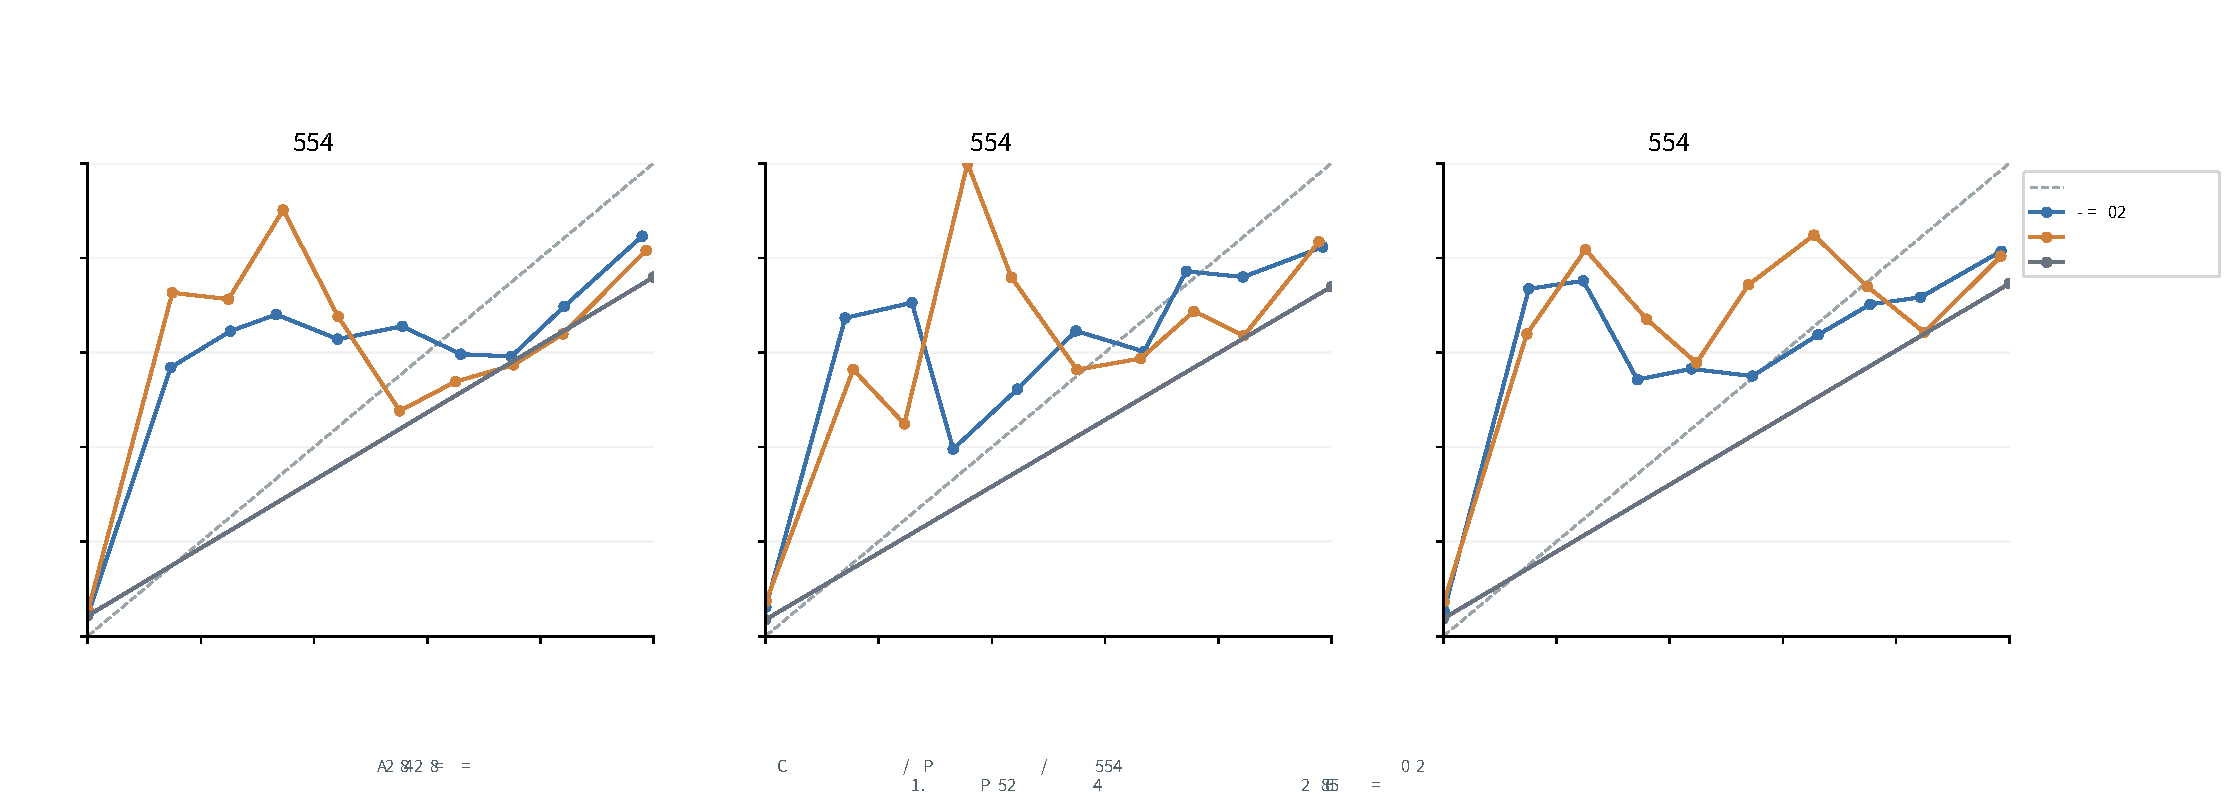
\includegraphics[width=.98\textwidth]{04_reliability.pdf}
\caption{Archived uncalibrated event reliability on the current 40-parent development cohort: one panel per seed, ten fixed bins, equal-parent weights. Empty bins are omitted; connecting lines are guides. Original Chinese labels are retained in this working-draft figure: ConPath (blue), independent (orange), deterministic (gray); horizontal axis predicted score, vertical axis observed event frequency. No fitted calibration curve or final-test result is shown.}
\label{fig:reliability}
\end{figure*}

\section{Results}
\subsection{Current Parent-isolated Development Evidence}
\begin{table}[t]
\caption{Current cohort only: 100/25/40 parent places, three seeds 20260910/11/12. Brier is mean $\pm$ sample SD. Risk30 is a mean at equal 30\% coverage. Missing rows are not zero. \valonly}
\label{tab:main}
\centering\scriptsize
\begin{tabular}{@{}lcrr@{}}\toprule
Method & Actual $K$ & Event Brier $\downarrow$ & Risk30 $\downarrow$\\\midrule
Deterministic occupancy & 1 & $0.11152\pm0.00256$ & 0.2516\\
Independent Bernoulli & 32 & $0.11201\pm0.00366$ & 0.2443\\
Direct-query & --- & Not evaluated & ---\\
No-global & --- & Not evaluated & ---\\
No-event & --- & Not evaluated & ---\\
ConPath & 32 & $0.10380\pm0.00350$ & 0.2395\\\bottomrule
\end{tabular}
\end{table}

ConPath has lower Brier than independent in all three seeds (Table~\ref{tab:main}). The independent-minus-ConPath difference is 0.00821, with archived source-stratified paired-parent interval $[0.00439,0.01251]$, conditional on the three seed means. Against deterministic occupancy the difference is 0.00772 with interval $[-0.01616,0.03377]$. Thus the available evidence supports the independent comparison, not a stable deterministic-baseline advantage.

ConPath's retrospective NLL and ECE are 0.79330 and 0.08622, versus independent's 0.94364 and 0.10131. At threshold 0.8, ConPath has risk 0.18649 at coverage 0.21340; independent has risk 0.20847 at coverage 0.22453. Lower risk at lower coverage is not a matched-coverage safety claim. The train-fitted radius prior has better NLL 0.48499 and ECE 0.05653, but higher Brier and zero threshold-0.8 coverage; its threshold risk is undefined.

Continuous hidden-map Brier is 0.15147 for ConPath, 0.15158 for independent, and \emph{better} at 0.13869 for deterministic occupancy. ConPath's free-space sample IoU is 0.62238 versus deterministic's 0.66228. Deterministic binary-map Brier must not replace its continuous Brier to manufacture a mapping advantage. A previously saved post-hoc fixed-0.5 conditional-mean-map control gives ConPath Event Brier 0.11410 and risk30 0.27791; it is distinct from the separately trained deterministic model.

Difficulty is uneven: a saved diagnosis finds 750/1,545 events forced unreachable by observations, with zero ConPath error. Its parent-weighted Brier on the hidden-completion-mutable subset is 0.19912. Easy known negatives therefore contribute to the low aggregate score.

\begin{figure*}[t]
\centering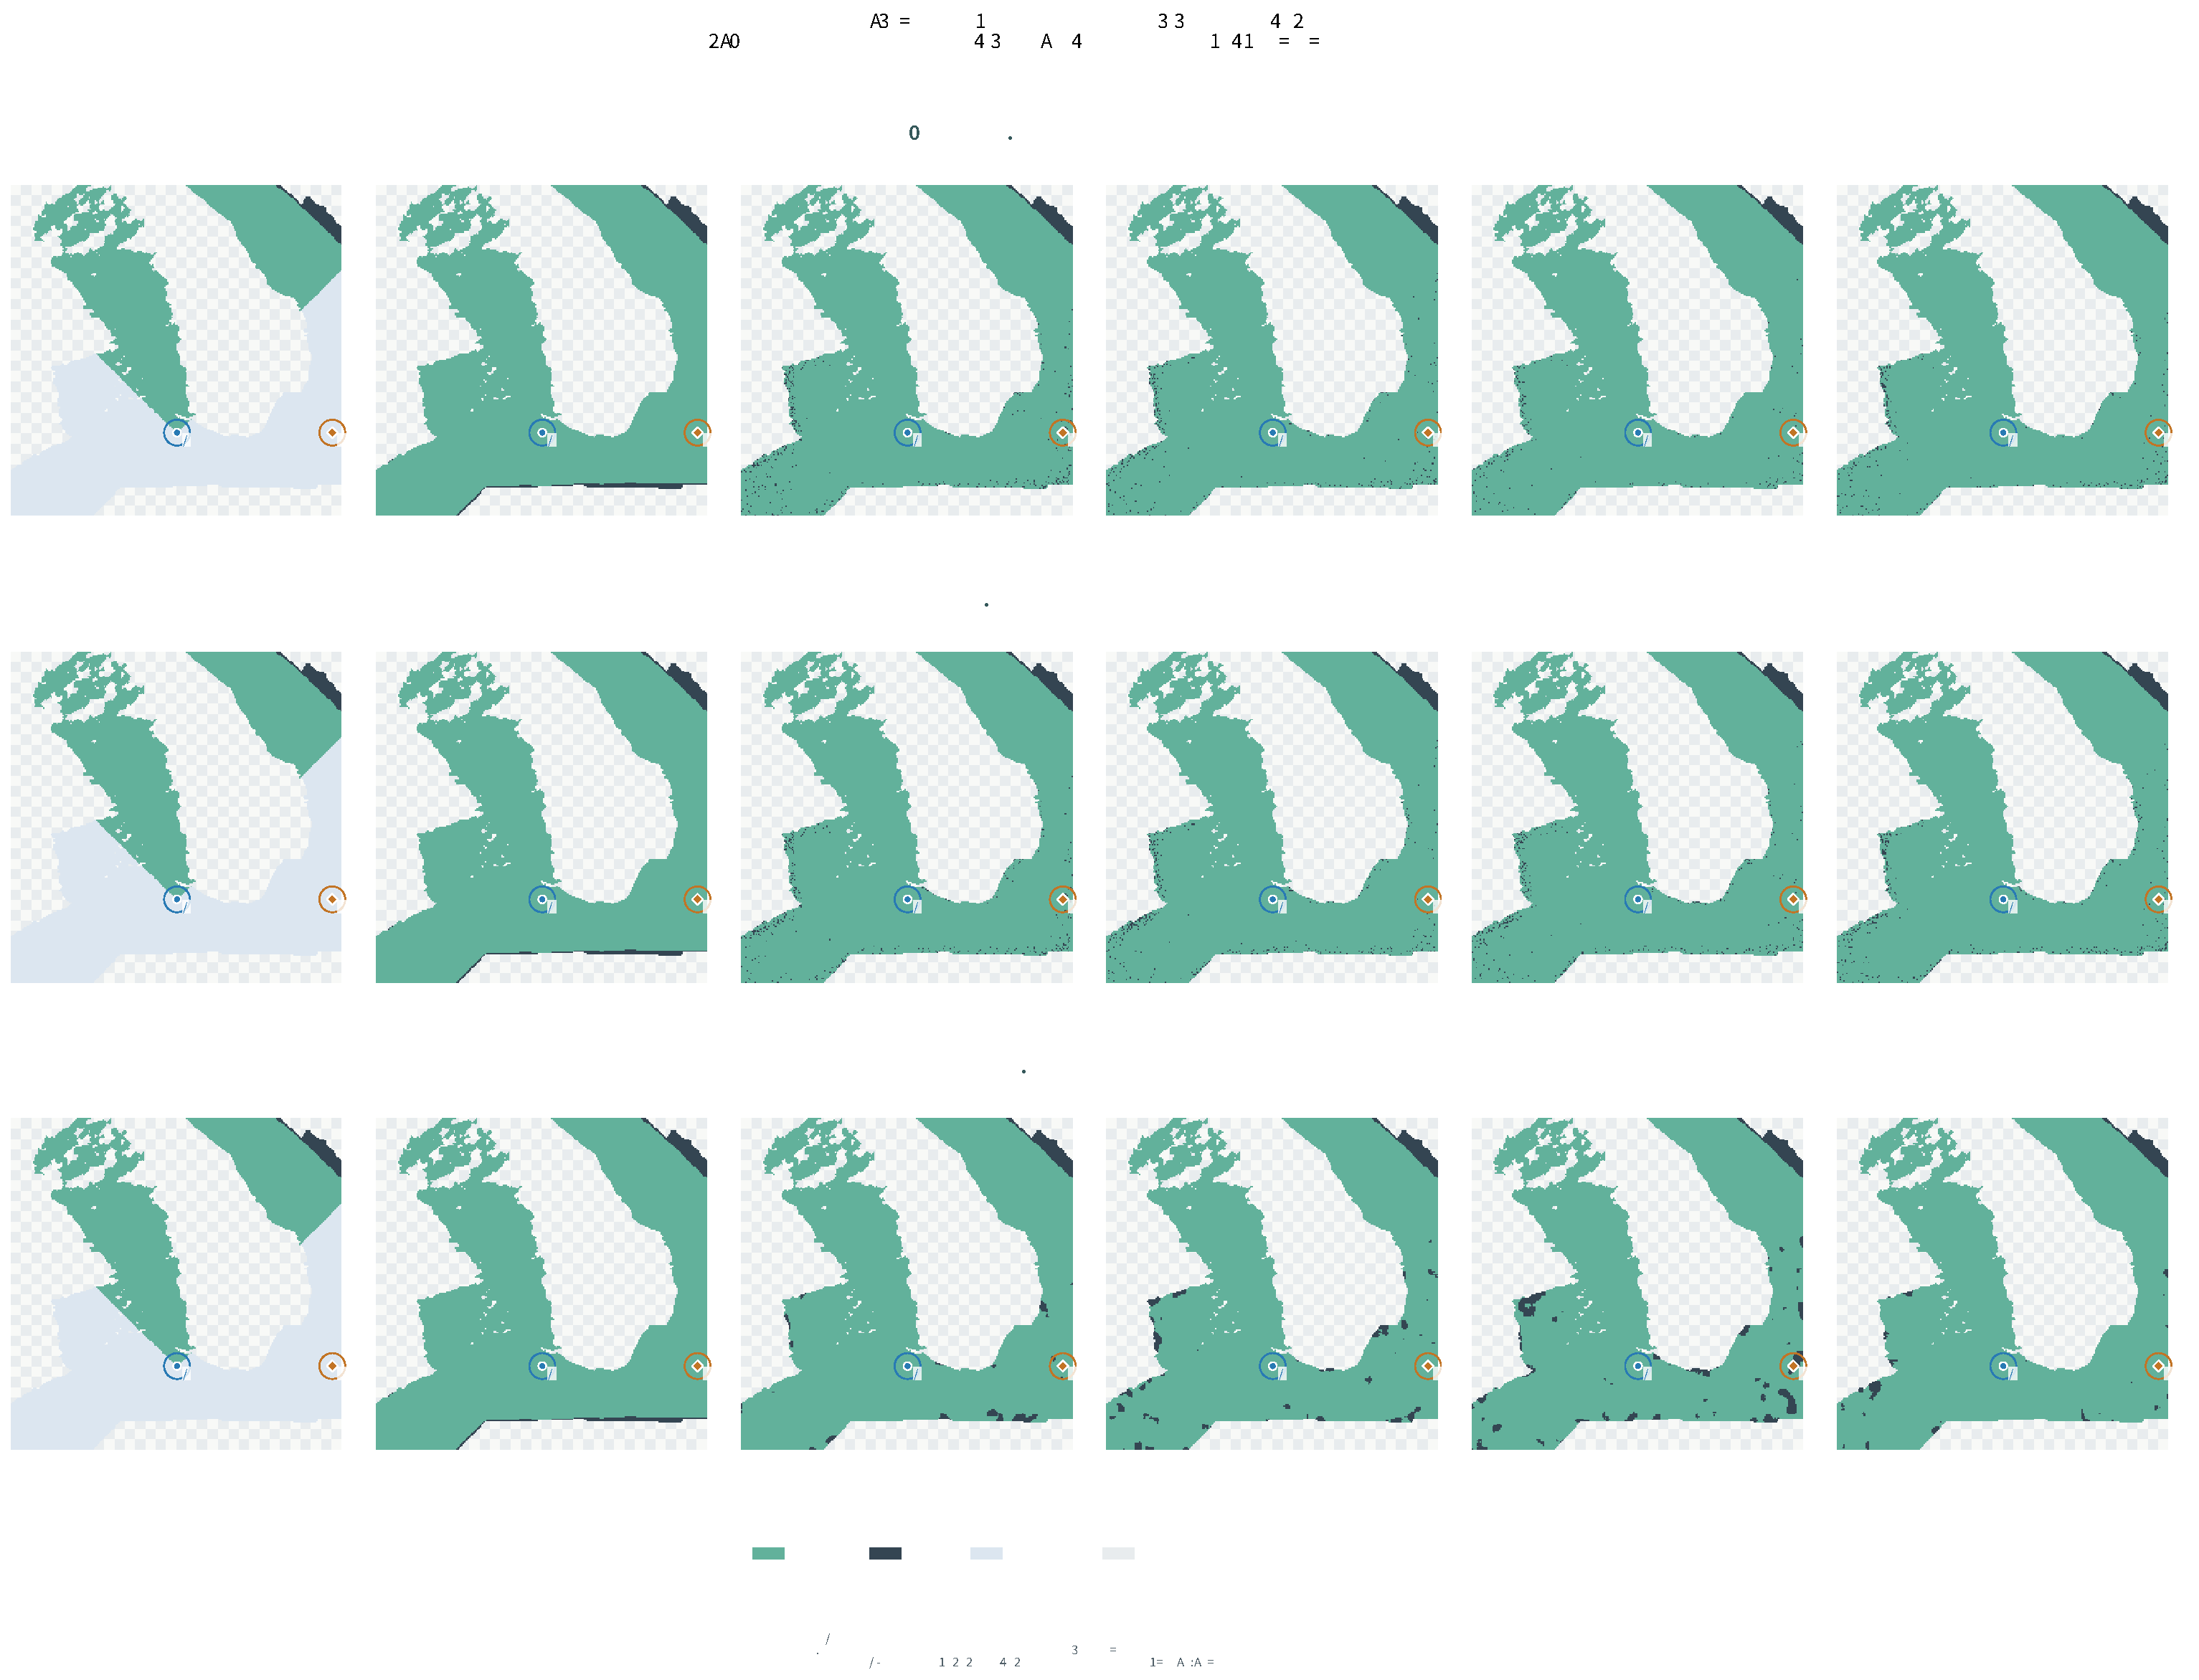
\includegraphics[width=.97\textwidth]{02_fixed_case_00.pdf}
\caption{First previously fixed case, \texttt{obs\_014028:q024}, seed 20260910, radius 10 cells, validation-only. Rows: original ConPath, independent, and a separately trained two-seed supplementary sampling variant. Columns: observation, reference, first four saved worlds; scores use all 32 worlds. Green is free, dark is blocked, pale blue is unknown, checkerboard is closed invalid support; S and G mark terminals, with footprint rings. The supplementary row is retained to preserve the unedited archived figure and is not the selected method. All ten cases appear in the supplement.}
\label{fig:case}
\end{figure*}

\subsection{RQ1 and RQ2: Historical Mechanism Evidence}
The historical fixed-marginal intervention independently permutes world indices at every cell of the saved $K=128$ ConPath ensemble. Every empirical free count remains identical, while sample alignment changes. Brier rises from $0.06749\pm0.00936$ to $0.16139\pm0.00677$. This isolates useful dependence in that finite ensemble, not the true infinite posterior or unseen-place generalization. Separately trained models do not constitute this strict marginal-matched test.

Historical no-event Brier, NLL, and ECE are 0.20425, 2.53067, and 0.21690; no-global obtains 0.09499, 0.78486, and 0.08592, versus full 0.06749, 0.28854, and 0.05715. Recorded within-seed subscene Brier intervals favor full. However, place overlap and event-based selection of no-event limit attribution. Historical direct-query has one seed and \emph{better} ECE 0.04076. The full same-checkpoint mean map has near-matching Brier 0.06957, with the direction reversing in one seed. These controls preclude broad all-metric stochastic superiority.

\subsection{Calibration, Selective Risk, and RQ3}
Figure~\ref{fig:reliability} preserves all three matched seeds. Historical equal-30\%-coverage risks are 0.03600 for full and 0.03901 for independent; every recorded within-seed paired risk interval includes zero. No-event has \emph{lower} threshold-0.8 risk 0.02561 versus full 0.04552, but lower coverage 0.19316 versus 0.33644. Neither threshold comparisons nor the historical ablations establish a robust safety advantage.



All 23 current method/seed/budget score files have zero radius-monotonicity violations across their 515 query triples. Existing saved-world audits report zero observed-evidence and support violations. These are structural checks, not a guarantee of empirical reliability. The historical no-event model predicts zero for all radius-20 queries despite a recorded 20.67\% positive rate, illustrating possible finite-footprint fragmentation.

Current ConPath Brier at radii 0, 10, and 20 is 0.15329, 0.09668, and 0.06142, respectively; independent obtains 0.16474, 0.10249, and 0.06880. Yet deterministic occupancy is better at radius 20 (0.04025), and ConPath accepts no radius-20 event at threshold 0.8 in any seed: its false-safe rate there is undefined. At radius 10 its mean risk is 0.30851 at coverage 0.03547, versus radius-0 risk 0.17754 at coverage 0.60473. The aggregate improvement therefore does not establish reliable high-confidence use for every footprint; these descriptive strata are tabulated in the supplement.

The qualitative set uses all ten previously fixed identifier-selected queries. Figure~\ref{fig:case} shows the first case in that list and the first four saved worlds in order; the displayed event forecasts use all 32. We preserve failures and unreachable cases rather than choosing attractive samples. No strict interior-bottleneck example survives the requirement that both terminals fit the footprint in this existing set. No current no-event/no-global sample arrays or preregistered occlusion sweep are available. RQ3 consequently has a structural monotonicity result and partial diagnostics, with explicit empirical gaps.



\section{Related Work}
\textbf{Mapping and planning.} MRFMap models occupancy dependence through forward ray sensor models~\cite{shankar2020mrfmap}; uncertainty-aware planning considers alternative path hypotheses~\cite{banfi2022uncertainty}. These precedents prevent novelty claims about correlated occupancy or uncertainty reasoning alone. ConPath scores a footprint-conditioned event from a supplied partial BEV.

\textbf{Connectivity supervision.} MALIS trains affinity graphs through maximin connectivity~\cite{turaga2009malis}, and learned promising-region methods supervise connectivity for sampling-based planning~\cite{ma2022connectivity}. Our contribution combines stochastic map inference, a footprint event, and a probabilistic score; the bounded gradient surrogate is not a new general maximin algorithm.

\textbf{Completion and calibration.} FlatLands studies deterministic and stochastic floor completion, including flow-based approaches~\cite{bhattacharjee2026flatlands}. LaMa uses Fourier convolutions for large-mask image inpainting~\cite{suvorov2022lama}. Our LaMa BEV adaptation and FM+XAttn literature reimplementation were stopped before adequate convergence and three-seed confirmation; neither is an official checkpoint or a formal main baseline. External mIoU, FID, and navigation-success numbers involve different datasets, tasks, outputs, and metrics and are not directly comparable to Event Brier. Proper and variogram scoring~\cite{gneiting2007proper,scheuerer2015variogram} motivate distinguishing marginal and dependence errors. Temperature scaling is established~\cite{guo2017calibration}, but is not fitted here; low ECE is not a safety certificate.

\section{Limitations}
All principal evidence is validation-only. The newer cohort is small, development-reused, bounded to at most 600 updates, and lacks three matched baseline families. Historical ablations have parent overlap and physical archive-test access; subscene intervals cannot be reinterpreted as independent-building uncertainty. Eligibility of an untouched final holdout is unresolved.

Inputs are supplied indoor BEV maps and valid-support masks, not end-to-end RGB/LiDAR. Outdoor generalization, real-robot closed-loop behavior, and control trajectories are not established. Discrete circular footprints and four-neighbor motion omit nonholonomic dynamics, arbitrary orientation, and continuous collision checking. Radius-to-meter calibration is unresolved. Finite ensembles and clipped NLL have numerical limitations, and training gradients are approximate. Deterministic controls remain strong; neither all-metric calibration nor uniformly better selective risk is supported. External generative models are not sufficiently converged formal baselines. Detailed gaps and source identities remain in the supplement.

\section{Conclusion}
ConPath connects joint stochastic maps to footprint-feasible path-existence forecasts. Current place-isolated development evidence improves on independently sampled completion, while separate historical interventions reveal the relevance of sample structure and event supervision. The evidence does not establish robust deterministic-baseline superiority, uniformly better selective risk, or final-test generalization. We freeze the original three selected checkpoints and stop additional tuning. The remaining paper decision concerns evidence sufficiency and a properly audited holdout, rather than further searches for marginal numerical gains.

\bibliographystyle{IEEEtran}
\bibliography{references}
\end{document}
